\documentclass[11pt]{article}
\usepackage{latexsym}
\usepackage{amssymb,amsmath}
\usepackage[pdftex]{graphicx}
% \usepackage{qtree}

\topmargin = -.75in \textwidth=7in \textheight=9.3in
\oddsidemargin = -.3in \evensidemargin = -.3in

\begin{document}
\begin{center}
\large
CS124 Programming Assignment 1
\end{center}
Joy Ming and Alisa Nguyen (05 March 2013)\\

\section{Data}
Our data for the average tree size for several values of $n =\text{number of vertices}$ is displayed in the table and graph below.
$$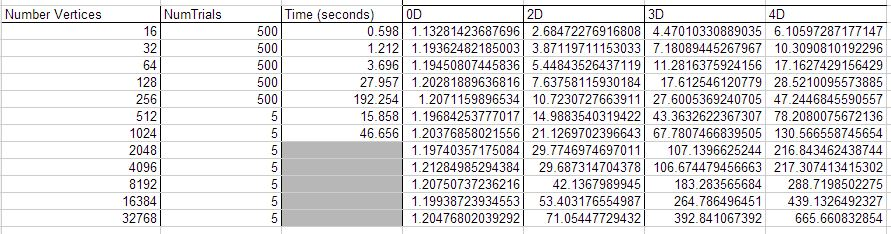
\includegraphics[width=180mm]{weightmsttable.jpg}$$
$$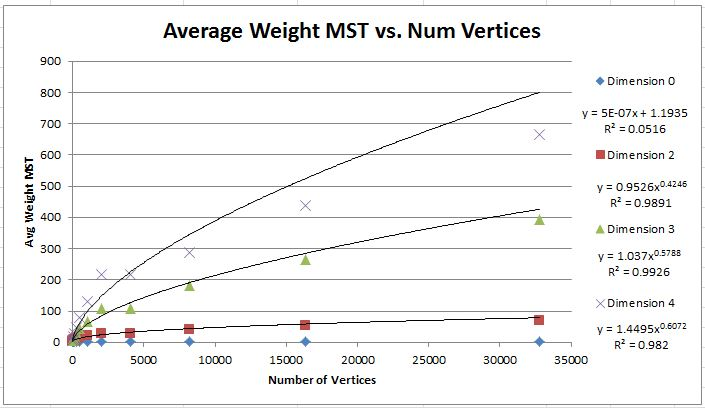
\includegraphics{weightmst.jpg}$$
\section{Our guess for function $f(n)$}
The growth rates for all the dimensions exept for 0D seem to be polynomial where the power is less than 1. More specific estimates of the growth rates we found are displayed on the graph and table below.
\begin{center}
\begin{tabular}{c c}
Dimension & $f(n)$\\
0D & $0.00007x + 1.1935$ \\
1D & $0.9526x^{0.4246}$\\
3D & $1.037x^{0.5788}$\\
4D & $1.4495x^{0.6072}$
\end{tabular}
\end{center}
For Dimension 0, we actually found an almost linear growth rate in which the average weight of the MST remains around 1.2 no matter how large $n$ grows. On the other hand, the other dimensions all grew with a power less than 1. However, our estimates for the growth rates do not look like they fit the points very well, and it seems as if our data beyond 8192 are skewed a little lower than they are supposed to for some reason. Although we tried to debug and many more trials on the large amounts of $n$, due to time constraints, we were unable to explore this phenomenon further and fix any possible errors related to these specific instances. Given more time and energy, we would return to figure out exactly what was going on for large numbers of $n$.
\section{Discussion of Experiments}
\begin{enumerate}
\setcounter{enumi}{0}
\item Prim's Algorithm
\newline
\newline
We chose to implement Prim's Algorithm because we wanted to practice implementing a minimum heap using the material we covered in leture and section. Actually implementing the heap in Java gave us a lot of practice with coding and debugging  in the language, since neither of us were too familiar with it to begin with. In terms of performance, we also believed that Prim's would work better in this situation because we are working with complete graphs with all possible edges, and since Prim's uses a priority queue instead of the simpler data structure used in Kruskal's to sort the edges, it would theoretically be faster.
\item Growth Rates
\newline
\newline
Initially, our data for the 0 dimension exhibiited a similar growth rate to the other dimensions, which we at first naively generalized as correct. However, upon further inspection of our implementation of Heap, we found that it was not in fact behaving as originally planned. So, after debugging and modifying our Heap, we finally received accurate growth rates for each of the dimensions, which are discussed more in depth in section 2. We were surprised that the growth rate for the 0 dimension graphs were so different from the other dimensions, but after discussing the way in which the Java Random library generates streams of random numbers, we realized that it made sense that the Gaussian distribution of the random weights would not cause the weight of the whole MST to increase by more than a constant factor over time.
\newline The growth rates seem to increase for higher dimensions, which is somewhat what we expected because there edge weights and the sizes of the MSTs also increase with dimension. However, because our data for large $n$ seem a bit skewed, we are unsure of the actual explanation for this.
\item Algorithm Run Time
\newline
\newline
The run time for our algorithm without pruning and simplifying graphs is charted below for the vertices in which we ran 500 trials. For number of vertices beyond 256, we ran 5 trials and the run times are listed in the table below. It makes sense that the run time grows almost exponentially because the number of edges grows exponentially without pruning as a function of $n$. Before simplifying the graph, running our algorithm on sizes of $n \geq 512$ would increase the CPU usage and slow down our computer's performance signficantly. The first times we tested our algorithm the program would run for upwards of 15 minutes before stopping or before burning out our computer and forcing us to restart. 
\newline
$$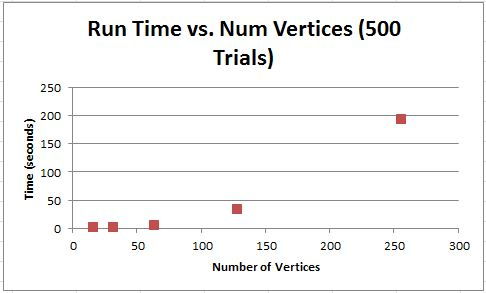
\includegraphics{runtime.jpg}$$
\item Random Number Generator
\newline
\newline
We used the random() function from Java's math library, which returns a long from 0 to 1 seeded by current system time. We didn't run into any interesting experiences using this method.
\item Simplifying our Graph for large $n$
\newline
\newline
We ran into quite a few issues dealing with large $n$ and tried many approaches throw away certain edges generated in the tree based on trends we saw in the data.
\begin{itemize}
\item First we tried throwing away edges that are heavier than the expected weight of a single edge in the graph we are considering simply based on a threshold calculation that was a function of only the dimensions of the graph. We had a cutoffs that were based on the hypercube line picking formula.
\item Then we realized that the cutoff should be determined not only based on the dimensions of the graph but also the number of vertices. We calculate expected weight by graphing datapoints of the longest edge in MSTs of each size $n$ for each of the dimensions, over many trials (500), and then finding a function $k(n)$ that best fit these data points, depending on the parameters $n$ and dimension $d$. The functions we came up with for each of the dimensions are shown on the graph below.
\newline
$$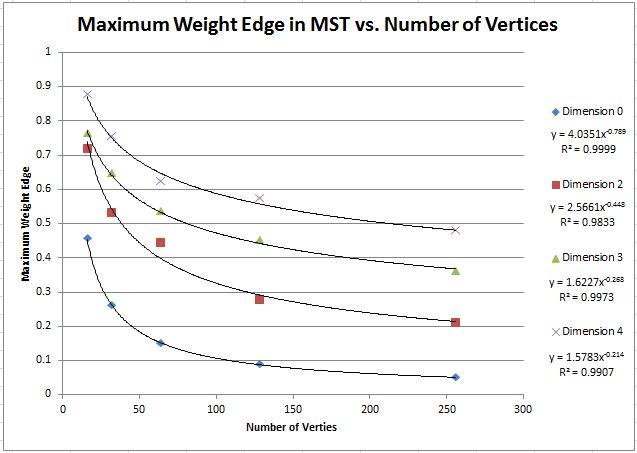
\includegraphics{prune.jpg}$$ 
\end{itemize}
To justify the correctness of these methods, because we are using complete graphs, there is a low probability that any edge higher than the expected weight will be chosen for the MST of that graph, as proven via trial and error. The table below shows our algorithm's performance with and without pruning for small numbers of $n$. There is no significant difference in performance.
$$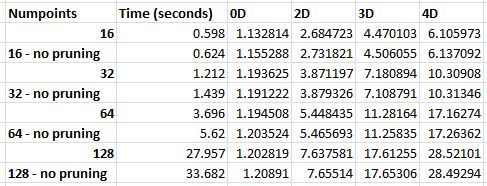
\includegraphics{pruning.jpg}$$
\item Handling large values of $n$
\newline
\newline
One aspect of this assignment we had the most trouble with was modifying our algorithm to be able to handle large values of $n$ in a short period of time. Although we tried many different methods to cut down on the running time of our algorithm and the space needed for large values of $n$, including limiting the amount of edges for each vertex to the minimum 30 because it is most likely that the edges for the MST will come from there, using a hash table to store our vertices and using an ArrayList of ArrayLists of Vertices, we were still unable to improve our running time by very much. Given more time and energy, we would continue to work through our method for generating the graphs to continue to remove unecessary pieces of information. From this assignment, we learned that space and time constraints are actually important and that we need to take them into consideration early on in the coding process instead of at the very end.
\end{enumerate}

\end{document}